\iffalse
\documentclass[journal,12pt,twocolumn]{IEEEtran}
\usepackage{graphicx}
\graphicspath{{./chapters/10/7/1/2/figs/}}{}
\usepackage{amsmath,amssymb,amsfonts,amsthm}
\newcommand{\myvec}[1]{\ensuremath{\begin{pmatrix}#1\end{pmatrix}}}
\providecommand{\norm}[1]{\lVert#1\rVert}
\usepackage{listings}
\usepackage{watermark}
\usepackage{titlesec}
\usepackage{caption}
\let\vec\mathbf
\lstset{
frame=single, 
breaklines=true,
columns=fullflexible
}
\thiswatermark{\centering \put(0,-105.0){
\includegraphics[width=0.75\columnwidth]{/sdcard/IITH/vector/chapters/10/7/1/2/figs/logo2.png}} }
\title{\mytitle}
\title{
Assignment - Vector
}
\author{Surajit Sarkar}
\begin{document}
\maketitle
\tableofcontents
\bigskip
\section{\textbf{Problem}}
Find the distance between the point(0,0) and (36,15).Can you now find the distance between the two towns A and B discussed in Section 7.2
\section{\textbf{Solution}}
\fi
Let
\begin{align}
\vec{A}&=\myvec{0 \\ 0}  
\Vec{B}=\myvec{36 \\ 15} \\ 
\implies 
\vec{d}&=\norm{\vec{A}-\vec{B}}=\sqrt{\myvec{\vec{A}-\vec{B}}^T\myvec{\vec{A}-\vec{B}}} \\
&=39
\end{align}
See Fig. 
\ref{fig:10/7/1/2vec}.
\begin{figure}[H]
\centering
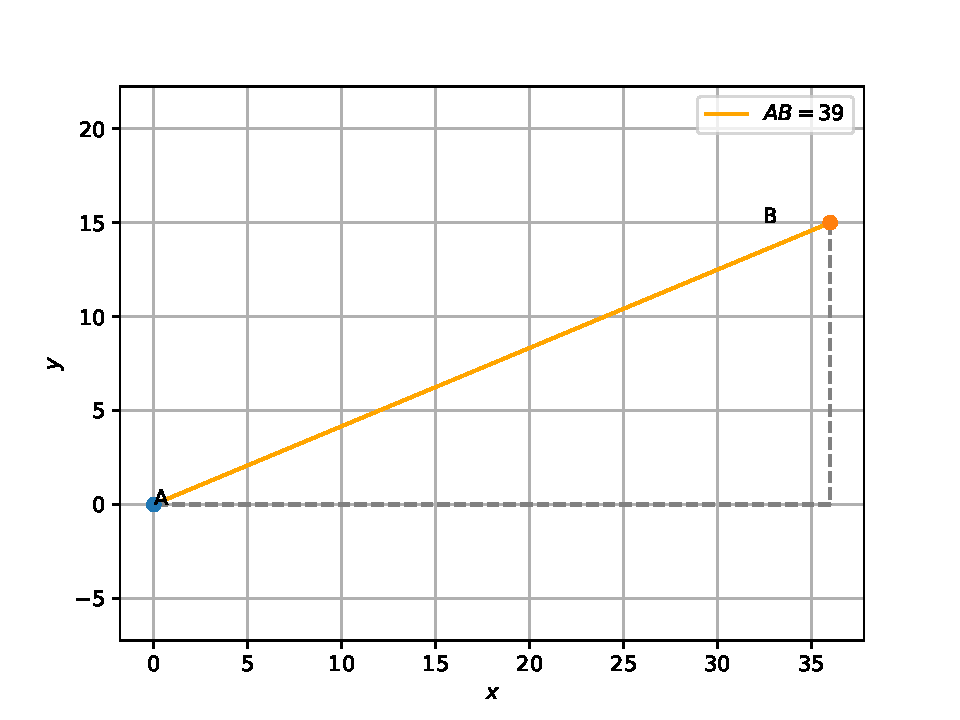
\includegraphics[width=0.75\columnwidth]{chapters/10/7/1/2/figs/vec.pdf}
\caption{}
\label{fig:10/7/1/2vec}
\end{figure}
